% id: 0549
% book: RPM 중3-2 수학 · 05 대푯값과 산포도
% section: 유형 04 여러 가지 자료에서 대푯값 구하기
% figure: crop:fig-0549.png
% answer: $48.7$
% answer_source: 답지
% variant_level: 0 (원본 전사)
% 이 파일은 build.mjs 가 items.json 에서 만든다. 고칠 때는 items.json 을 고친다.
\dmkichul{RPM 중3-2 수학 0549번 · 87쪽}
\noindent\begin{minipage}[t]{0.58\linewidth}\vspace{0pt}\raggedright 오른쪽 줄기와 잎 그림은 어느 중학교 3학년 학생 10명의 던지기 기록을 조사하여 나타낸 것이다. 이 자료의 평균을 $a\,\mathrm{m}$, 중앙값을 $b\,\mathrm{m}$, 최빈값을 $c\,\mathrm{m}$라 할 때, $a+b+c$의 값을 구하시오.\end{minipage}\hfill\begin{minipage}[t]{0.4\linewidth}\vspace{0pt}\centering 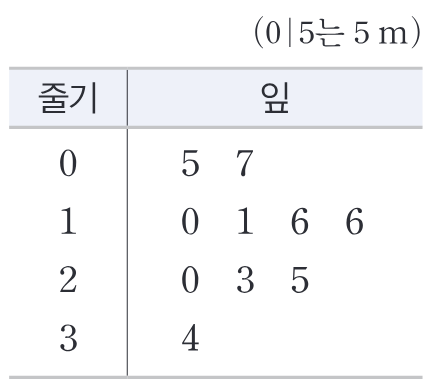
\includegraphics[width=103.2pt]{figures/fig-0549.png}\end{minipage}\par
